%%-*-latex-*-

\section{Related Works}

Recursion is well known among computer scientists for being difficult
to teach. Many have been the studies that tried to find efficient ways
to teach the concept. Also, tangible interfaces are subject to more
concrete investigations, that usually conclude with working
prototypes. The following is an attempt to summarize both approaches.

%*******************************************************************************
\subsection{Difficulties with Recursion}
%*******************************************************************************

Several mental models of recursion were inferred by different
studies~\cite{SandersGalpinGotschi:2006, Mirolo:2009} which brought
to the fore failures in understanding the concept. This approach is
related to the field of \emph{cognitive sciences} as it states that
the problem lies in the way novices mentally model the undergoing
process of a recursive function call.

The \emph{looping and copies models} identified by
Kahney~\cite{Kahney:1983} are known for being the most common
occurrences. The \emph{looping model} is present when recursion is
seen as an iteration that terminates when the base case is reached.
Students that think within this model have serious difficulties
understanding problems that can not be solved by evaluating the
solution at the base case, that is, calls which are not in tail form.
On the other hand, the \emph{copies model} presents a correct mental
representation of general recursion. This model is based on Kahney's
definition of recursion~\cite{Kahney:1983}:
\begin{quote}
  Recursion is a process that is capable of triggering new
  instantiations of itself, with control passing forward to successive
  instantiations and backward from terminated ones.
\end{quote}
In this model, forward and backward control flow are correctly
identified and explicitly shown. Further
evidences~\cite{GotschiSandersGalpin:2003, SandersGalpinGotschi:2006,
  Kahney:1983, George:2000a, Wu:1993} sustain that this is the
correct path to follow since it represents a simplified and clear
view of recursion's internals as experimented by experts.

Other nonviable models are linked to frequent problems exhibited by
beginners. Some of these models, such as the looping model and the
\emph{active model}, where the active flow control is identified, are
sometimes found in experts~\cite{GotschiSandersGalpin:2003} in
combination with the copies model because they are partially correct
as they abstract forward control flow. However, the lack of backward
control flow understanding make them inadequate for most of the
situations. Other models lack any understanding of recursion and will
mostly never lead to correct solutions. These
models~\cite{GotschiSandersGalpin:2003} are: the \emph{step model}, where
the student executes the recursive condition only once; the
\emph{algebraic model} where the student tries to apply mathematical
concepts; the \emph{return model} where he believes values are to be
generated and stored by each recursive call and finally combined to
give a solution; and the \emph{magic model} where the student knows the
language syntax but has no comprehension of the semantics. Finally,
as sad as it is, many students possess the \emph{odd model}. In this
model, many misunderstandings are present, thus,
novices find themselves unable to predict simple program behaviors.

These mental models are cognitively linked to individual's learning
styles, therefore, different mental models of recursion could be
more effective for different learning
styles~\cite{WuDaleBethel:1998}. This is specially visible on
students who build their knowledge based upon speculations and
previous knowledge. More investigation must be focused on finding
the possible matches between learning styles and conceptual models.

Another studied possibility is related to the correct identification
of base cases~\cite{HabermanAverbuch:2002}. In this setting,
students handle redundant base cases, and ignore important cases such
as boundary values, degenerated cases, out\hyp{}of\hyp{}range values.
In the worst occurrences, they may even not define any base cases when
formulating recursive algorithms. This situation leads to incomplete
solutions and thus cause incomplete understanding of the concept.

Focusing on the linguistic nature of the communicative interaction when
learning, Levy proposes the use of English language as a tool to describe
recursive concepts~\cite{LevyLapidot:2000, LevyLapidotPaz:2001,
  LevyLapidot:2002, Levy:2001}. He performs an experiment in which
freshmen of business majors are asked to describe with words the
recursive procedures taking place in an imaginary service
corporation. The main conclusion obtained with this experiment is
that programming without a programming language becomes easier,
because the function of both the program and the programming language
is better understood with words. This work leads to the proposal of
a methodology to better understand recursive programming based on the
notion that the concepts ``process'', ``program'' and ``processor'' are
fundamental in computer programming~\cite{LevyLapidot:2000}. Thus, a
proper explanation of these terminology to beginners improve their
understanding of the whole picture.

In a related work~\cite{Kimura:1977}, the student's discourse is
analyzed, as a step toward understanding the students ways of speaking
recursively. Preliminary results indicate the existence of some basic
aspects of recursion in the student's discourse, although the students
apparently talk a very different language from that of the experts,
as used by books and teachers. This study underlies the linguistic
nature of computer programming. Their conclusions are of vital
importance, for linguistics is the foundation of the communication
between the teacher and the student.

Even though computer scientists learn and practice recursion in
several courses of many universities, they rarely rationalize or
use recursion as a problem solving means. During an
experiment~\cite{Ginat:2004}, students are given three algorithmic
tasks, for which the most suitable solution approach is recursive.
Student's solutions and explanations demonstrate very limited
capitalization on recursion as a problem solving technique.
Explanations of this issue are related to the lack of assimilation
of recursion as a general reasoning and problem solving method.
Another explanation lies in the fact that recursion is usually
taught in schemes that are tied to very particular computations,
such as tree and graph traversals.

The mathematical principles behind recursion have also been brought
to the fore in very diverse and ingenious approaches. Many authors
insist on the close relation between recursion and mathematical
induction~\cite{LeronZazkis:1986, BrandtRichey:2004, Polycarpou:2006}.
Some others compare the intrinsic recursive behavior of certain
mathematical concepts such as \emph{Fibonacci
  numbers}~\cite{RubioHernan:2007} or the \emph{factorial
function}~\cite{Wu:1993}. The importance of a good mathematical
background that students must obtain in high school is also
highlighted by daRosa~\cite{daRosa:2002} who identifies the origin
of the recursion difficulties in novices as a side effect of poor
mathematical grounding. To conclude, she suggests to improve the
teaching of discrete mathematics in high school curricula.

In a similar manner, the teaching of recursion and lists before
iteration and arrays has also been discussed. A
study~\cite{TurbakRoydenStephanHerbst:1999} is based on the fact
that logically and pedagogically iterative procedures can be
presented as a particular pattern of recursion. On the other hand,
another study~\cite{BruceDanylukMurtagh:2005} is based on the
reinforcement that recursion provide, in order to define and use
objects and classes. In this approach, students with an early
presentation of recursion are reinforced in the fundamentals of
classes and as a consequence they appreciate the reasons to use them
to encapsulate data access and modification.

%*******************************************************************************
\subsection{Remedies}
%*******************************************************************************

The mentioned difficulties have made recursion an issue to worry
about by programming teachers. The lack of an everyday analogy of
recursion puts the student in a situation where he can not compare
the concept with any previous knowledge. On the contrary, arrays
and loops are observed everyday in the form of general tasks like
repetitive processes, items counting, object grouping, etc. However,
some infrequent objects such as tree branches, various vegetables
like the cauliflower and the broccoli, \emph{fractals figures} and
certain kinds of art (most notable by Escher) could be interpreted and
described in a recursive manner~\cite{LevyLapidot:2002}. Gary Ford
conducted an experiment~\cite{LevyLapidot:2002} where a group of
students had to construct recursive descriptions of some of the
previously mentioned phenomena. He theorized that their correct
understanding might help novices in the later construction of more
formal recursive descriptions using a programming language by creating
analogies between the real and the programming scenarios. His results
lead to the conclusion that learners and educators awareness of both
the \emph{building blocks} of any recursive description and the
several possibilities for assembling these blocks, might help in the
process of understanding recursion in general, and in particular in
the further construction of recursive functions. As a consequence, we
can think that recursion is probably easier to teach by explaining how
it appears in these objects because students are able to visualize the
process. Based on this assumption, new recursion problems have been
proposed. One of these problems~\cite{Wirth:2008} consists in randomly
parking cars along a street which could be taught in programming
courses as solvable by a scheme called
\emph{divide\hyp{}and\hyp{}conquer} which consists in giving a
solution as the mix of sub\hyp{}solutions. The problem could also be
used to introduce the concept of \emph{stack} and to show that several
problems are easier to solve by using recursive calls as opposed to
using loops.

Another study~\cite{Velazquez:1999} is based on the assumption that
the difficulty in learning recursion does not come from the recursion
concept itself, but from its interaction with the mechanisms of formal
grammars, functional programming and imperative programming.
Consequently, recursion is introduced in a gradual way by means of
its instances in the three frameworks and then each instance of
recursion is explained so that all of its accompanying mechanisms are
clearly identified~\cite{Velazquez:2000}. Students clearly identify
recursion as a frequent concept in computer science and not just as a
part of imperative programming.

In order to help students to grasp the concept, several authors have
proposed a set of abstract ways. Haynes~\cite{Haynes:1995} identified
several approaches such as the \emph{inductive definition} that
explains how the function is defined in terms of itself and base case;
the \emph{run\hyp{}time stack}, that consists in seeing recursion as a
process of pushing and popping stack frames; the \emph{trace}, where
every time a procedure is called, a line with the procedure name and
the input parameters are printed and, every time a procedure ends, a
line with the procedure name and return value is printed out.
Additionally, he proposed a new approach called the \emph{activation
  tree}, which is a conceptual combination of the run\hyp{}time stack
and the recursion tree. In this methodology, the stack frames of the
run\hyp{}time stack contain additional information from the recursion
tree that makes it easier to follow the dynamic execution of the
program. Students are found the activation tree to make recursion
clearer. This kind of solutions has an important impact as it guides
the teachers and provides them with different ways to convey the
concept to the class.

Graphical approaches are also very relevant. The first line of
investigation started as graphical techniques to pedagogically
describe recursion. One of the early works~\cite{Jackson:1976}
pictures recursive procedure calls by a method that uses a form of
self\hyp{}generating state diagram. This approach enabled the student
to visually keep track of where program control is located at each
moment during execution. Another visual
modeling~\cite{SternNaish:2002b} consists in classifying recursive
algorithms according to two criteria: the way they move across a data
structure and the way they manipulate items within it. These
approaches, in conjunction with the abstract ways of considering
recursion, are relevant conceptual tools for teachers.

Interactive solutions also have been proposed. One of them is the
study of a simulation of \emph{recursive traversals} of binary
trees~\cite{KurtzJohnson:1985}. Students who participate in this
simulation can be divided in two groups: the ones who understand the
relation between recursive pseudo\hyp{}code and the information
displayed and a few others who adopts the \emph{survival strategy}
of keeping hitting keys until they are finished. According to
posterior results, the second group of students seems to have learned
about tree traversals. However, they do not gain the more substantive
recursive understanding of relating the pseudo\hyp{}code with the
graphic display. In a similar manner, a second
approach~\cite{ChaffinDoranHicksBarnes:2009} provides the computer
science students with the opportunity to write code and perform
interactive visualizations. The game challenges the student to
complete three puzzles in order to learn about recursion through
the \emph{depth\hyp{}first search} of a binary tree. After completing
the game, most students exhibited a growth in their learning and a
very enthusiastic attitude towards learning games and how they are
built. The authors of these visual experiences emphasize the good
results during their teaching sessions as digital games have proved to
be adequate for learning~\cite{Nelson:1962, InbarStoll:1970,
  Prensky:2003}.


%*******************************************************************************
\subsection{Tangible User Interfaces applied to didactics}
%*******************************************************************************

The application domain of tangible interfaces is very wide. Their
popularity has increased during the lasts two decades. Specially
noticeable is how children are playfully attracted to this kind of
interfaces. Consequently, researches have created a series of
game\hyp{}like tangible interfaces for learning~\cite{EEMB:2009,
  Marshall:2007, PRSSN:2003, RSGSH:2002}.

Children are not the only ones benefited. Several other studies have
shown equally comparable results in people with learning disabilities
or novices of any kind~\cite{ZuckermanAridaResnick:2005}. Another
study that relates the interaction between live music performance and
tabletop tangible interfaces~\cite{JGAK:2007} demonstrates that both
adults and children can be equally aided by tangible artifacts.

\begin{figure}
  \centering
  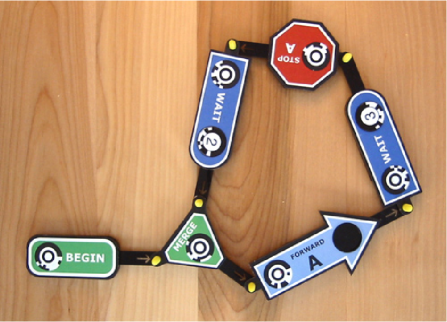
\includegraphics[width=0.6\textwidth]{img/relworks/tern.png}
  \caption{Example Tern statement~\cite{HornRobert:2007}}
  \label{fig:tern}
\end{figure}

Another study~\cite{HornRobert:2007} developed and analyzed a visual
language called \tern. This language is based on the text\hyp{}based
programming language described in the book ``Karel the Robot: A Gentle
Introduction to the Art of Programming''~\cite{Pattis:1994}. In \tern,
students connect wooden blocks shaped like jigsaw puzzle pieces, shown
by~\fig{fig:tern}, form flow\hyp{}of\hyp{}control chains for
elementary virtual robots in a grid world displayed on a computer
screen. Students cooperatively design and create programs on their
desks or on the floor by connecting pieces among each other. These
pieces were scanned by a portable station and a reliable computer
vision software in order to compile the abstracted code. This visual
tool is of special help to incite students towards collaboration. They
program multiple robots that can interact in the same world. Several
teams of students work together to solve the proposed challenges that
include collecting objects and navigating through a maze.

\begin{figure}[h!]
  \centering
  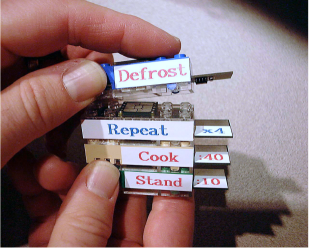
\includegraphics[width=0.6\textwidth]{img/relworks/bricks.png}
  \caption{Tangible programming bricks~\cite{McNerney:2000}}
  \label{fig:bricks}
\end{figure}

Similar to the later, tangible programming bricks~\cite{McNerney:2000}
are physical building blocks for constructing simple programs. These
bricks, which can be observed in~\fig{fig:bricks}, prove to be useful
for controlling diverse objects such as toy cars or kitchen
appliances. This interface brings down the wall that divide
programmers from non\hyp{}programmers by allowing children and novices
to create their own controlling software. The users are encouraged to
adopt it because the bricks are easier to use than text editors, help
to explain to others their programs and to remember better their
programs in comparison to traditional programs.

\begin{figure}
  \centering
  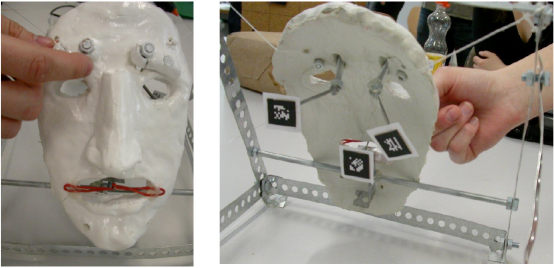
\includegraphics[width=0.8\textwidth]{img/relworks/ar_proto.png}
  \caption{Augmented Reality prototype~\cite{HorneckerPsik:2005}}
  \label{fig:arproto}
\end{figure}

Finally, \emph{augmented reality} (AR) plays an important role in
didactic interfaces. A substantial work has been developed by a group
of teachers and students who created a technique for quick prototyping
of tangible interfaces based on AR~\cite{HorneckerPsik:2005}. The
students creatively adapted optical \artoolkit markers for a class on
experimental prototyping of tangible appliances. The markers are used
to visually track the position of objects, with the advantage of a
wide variety of interactions as the one shown in~\fig{fig:arproto}.
Another work~\cite{Billinghurst:2002} combines the idea of a virtual
guitar assistant with AR. The remarkable part of the system is the
visual warnings displayed when invalid notes are played.

\constructd is a ``three dimensional geometric construction tool
specifically designed for mathematics and geometry
education''~\cite{KaufmannSchmalstieg:2002}. The main contributions of
this research lies in the collaborative environment created around the
interaction of the augmented reality appliances and the concrete
implementation of a virtual 3D scenario for 3D objects. Initial
evaluations show that students work in a constructive manner within
only a short delay. Even though the system has not been deployed in a
production environment, these preliminary results encourage researches
towards the development of augmented reality interfaces with educative
purposes.
